\chapter{Background}


The main idea of our project is providing a paraphrasing feature within a Computer Aided Translation system by reusing the information that is available as a result of machine translation process which output is used to provide user with an initial translation. Before introducing our approach, we would like to provide some background information about CAT systems, relationship between paraphrasing and translation tasks as well as some concepts of machine translation that were are used by our approach to implement paraphrasing.  

\section{Computer Aided Translation}

Recently, more and more papers discussing various aspects of Computer Aided Translation are published. This increase could be explained by the fact that the need of high quality and publishable translation is still satisfied by human translators and how advancements in machine translation are efficiently used by them in order to increase productivity of translators is still an open question. Various ways of assistance were suggested and implemented. Most of these tools are reportedly increasing translation speed, others help to achieve a better quality. In this work we present a novel assistance type, which aims to help translators by providing with paraphrases - alternative ways of expressing the same ideas. Before discussing paraphrasing, we want to highlight the ways our approach could be used in the context of CAT systems that provide different types of assistance.


\subsection{Interactive Machine Translation}

One way to assist translators is providing auto-completion suggestions while he composes the translation in target language. As user's input in text editor component changes, system suggests possible translation of the following word or phrase. The first system implementing this approach was TransType (Langlais et al., 2000; Foster et al., 2002; Bender et al., 2005), providing optional sentence-completion suggestions based on machine translation.  Based on user's acceptance of the suggestions, system can be improved to provide better results (Barrachina). Caitra is another CAT system described by \cite{KoehnHaddow2009} which also provides an interactive mode, where system uses search graph of machine translation decoder to suggest multiple options for upcoming words and phrases translation. 

Our paraphrasing approach similarly reuses search graph for generation of alternative translation options, however in contrast to Interactive Machine Translation systems we assume that the user already has an initial translation, that she wants to improve using better wording. This initial translation could be originally produced using an interactive assistance with auto-completion or alternatively it could be a result provided for post-editing.

\subsection{Post-Editing}

Another popular assistance way is providing machine translation for post-editing by translator. In this case for each sentence in the document that is being translated, multiple translation options are provided. User can select one by clicking on it, what will update value of text editor component with the chosen translation. Alternatively, user can ignore suggested options and start typing translation manually and possibly she can take advantage of an aforementioned interactive suggestions.  

Effect of post-editing on productivity of the translation process was analysed by many researchers, including (...). It was previously demonstrated that post-editing can significantly improve performance of translator in some contexts like legal and information technology documents (...). However, in other domains like news and media, initial translation produced for post-editing is far from publishable quality. This output is being manually fixed and improved, by replacing erroneous parts with correct words preserving the meaning. This is one of the situations when our assistance paraphrasing service aims to help user to find multiple possible alternative translations of the corrupted part.

During this project we were investigating feasibility of our tool, in scope of a CAT system that provides post-editing options. However, our approach requires only information generated during machine translation decoding, the search graph, which is also being build during interactive translation. That means our technique could be easily extended to be used with the CAT systems without post-editing, that provide machine translation driven assistance by other means.

\subsection{Bilingual concordancer}

Bilingual concordancer is a feature used by professional users to explore alternative translations of particular phrases. This is achieved by finding occurrences of the phrase in bilingual corpus and retrieving their corresponding translations. Analyses of usage logs of TransSearch, one of the most popular bilingual concordancers, for 6 years demonstrate that tranlators find this feature useful especially for finding the correct sense in case of highly polysemous adverbials and prepositional phrases \cite{Macklovitch2008}. We believe that our paraphrasing tool that given one possible translation of a phrase explorers other alternative translations might be also useful in terms of finding a translation that preserves the meaning of the original phrase in a better way. We expect that starting the search within the same language, will simplify the this task for users with poor understanding of source language.


\subsection{Other assistance ways}

Providing various translation options for parts of sentence in source language, can also help in translation task. As it was shown by \cite{Koehn2010}, using this assistance it is possible to achieve translation with acceptable quality without understanding source language. The difference of our approach is that instead of providing different translation options for parts of original text, we produce paraphrasing options for any user specified parts of translation. This similarly to translation options, our tool can be used by someone, who doesn't know original language, to understand unclear parts of the text provided for post-editing, by paraphrasing them into representations that make more sense to him.

Finally, feasibility of our approach could be improved when used together with other CAT features like idioms and terminology detections. Indeed, having idioms or terminology marked in user's input for paraphrasing they could be treated in specific ways. In case of terminology paraphrasing lookup might take benefits of domain specific thesauruses. For idioms, paraphrasing algorithm will consider them as atomic units and will not try to paraphrase them partially. 

\subsection{Summary}

In conclusion, we described how assisting translator by providing paraphrases of translation could be used together with other assistance means provided by a CAT system. While our implementation requires data generated by a translation decoder, this data is not supposed to be generated separately specifically for paraphrasing needs, but rather data available after running translation system for an interactive assistance or post-editing could be successfully reused for paraphrasing. We also compared our approach with tools like bilingual concordancer and translation options provider, highlighting similarities and differences. And finally, we mentioned how paraphrasing could take advantage of idiom and terminology detectors.

\section{Paraphrasing Approaches}

Here we will summarize outcomes of this and variety of other data-driven paraphrasing techniques previously available in the literature. Essential difference of our approach from the ones listed in this section is that while most of previous studies were focused on paraphrasing generation problem, trying to extract paraphrases from various sources and store them for future usage, our approach is considering paraphrasing as search problem and aims to find paraphrases for a phrase that is given in a context of a sentence that is being translated by a user. Despite this difference ideas from these approaches were used by us for achieving better results and for developing an automatic evaluation approach that was useful for assessing multiple versions of our paraphraser. 

\subsection{Data-driven paraphrasing}

Originally paraphrasing was considered within multiple problems in Natural Language Processing, including question answering, summarization and generation. As a result historically there were multiple approaches for paraphrasing including techniques using formal semantic representation and methods that used grammars. More recent approaches are statistically motivated and make use of various data sources to generate paraphrases. 
Main data sources that were used in previous literature include multiple translations (for example multiple translations of classical literature), comparable corpora (news articles about same events, different encyclopedia articles with same subject), and monolingual corpora (in this case distributional similarity is exploited to find paraphrases). A novel technique introduced by \cite{Callison-Burch2007}, describes how bilingual parallel corpora could be successfully used for paraphrase generation, this approach is related to the technique we use for paraphrasing. Similarly, the data we exploit is build during a statistical machine translation process and derives from a bilingual parallel corpora.

\subsection{Multiple translations}

The key idea of the techniques that exploit multiple translations as a data source for paraphrase generation is that translators composing different translation of the same text were preserving it's original meaning, what makes these translations natural sources for paraphrasing (). First experiments with multiple translation of French classical literature were focused on extracting paraphrases by detecting different phrases in similar contexts. So for example, following French sentence, might be translated into English in two different ways as follows:

\begin{center}
\begin{Large}
\textbf{G\`{e}n\`{e}ralement, les gens qui savant peu parlent becoup,\\ et les gens qui savant beaucoup parlent peu}
\\
\small{\textit{(Jean-Jacques Rousseau)}}
\end{Large}
\end{center}

\begin{center}
\begin{Large}
People who know little speak a lot, and the people who know a lot speak little. 
\end{Large}
\end{center}

\begin{center}
\begin{Large}
People who know little are usually great talkers, while men who know much say little.
\end{Large}
\end{center}

Aligning similar parts of both sentences, we can see that ``are usually great talkers'' and ``speak a lot'' appear in same context and therefore they probably have same meaning.

Later researchers applied more complex ways to detect paraphrases in multiple translations, this includes using parse trees and considering parts of sentence with similar syntactic role to be paraphrases.

While our paraphrasing approach doesn't exploit this ideas. We used similar technique to develop an automatic paraphrasing evaluation framework. Instead of multiple translations that are rarely available we used a machine translation to corrupt natural language sentences, and later used difference between original and corrupted sentences as paraphrasing target. This technique similarly decides whether parts represent same idea or not by considering the surrounding context. Our evaluation methodology will be discussed in detail in Chapter 5.

\subsection{Bilingual parallel corpus}

Close ties between paraphrasing and translation were studied by \cite{Callison-Burch2007}. The results of this work were important for designing our paraphrasing approach. 

In contrast to previous studies that use monolingual data as main source for paraphrase detection, technique described by \cite{Callison-Burch2007} exploits parallel corpus that contain text in two languages. Previously, this data has been considered mostly for solving statistical translation task. Authors demonstrated that similar statistical approach could be applied for solving paraphrasing problem as well.

In case of multiple translations and comparable corpora aligned equivalent sentences were detected and used as natural source for paraphrasing. However, this technique that deals with sentences paired with their translations, uses an alternative approach. It finds paraphrases using multiple occurrences of same foreign phrase that has different translations as pointers to possible paraphrases. Indeed, if two phrases have same translation in a given number of cases, they are probably encoding same meaning.

The main idea could be illustrated in terms of probabilities. Let's define paraphrase probability as $p(e_{2} | e_{1})$, which designates a probability of that phrase $e_{2}$ is suitable paraphrase for given phrase $e_{1}$. This probability is defined similarly to the translation model probability $p(f | e_{1})$, which expresses probability of that foreign phrase $f$ has same meaning as given original phrase $e_{1}$. Another required expression is $p(e_{2} | f)$, the probability of that phrase $e_{2}$ is translation of given foreign phrase $f$. Considering that original phrase $e_{1}$ that we are trying to paraphrase may have multiple foreign translations, for the final expression paraphrase probability we will sum over $f$.

\begin{large}
\begin{equation}
\hat{e}_{2} = \arg\max_{e_{2} \neq e_{1}} p(e_{2} | e_{1})
\end{equation}
\end{large}

\begin{large}
\begin{equation}
\hat{e}_{2} = \arg\max_{e_{2} \neq e_{1}} \sum_{f}p(e_{2} | f)p(f | e_{1})
\end{equation}
\end{large}

\begin{center}
\textit{\cite{Callison-Burch2007}}
\end{center}

In equations \textit{(2.1)} and \textit{(2.2)} $\hat{e}_{2}$ represents the most probable paraphrase for originally given phrase $e_{1}$. Multiple ways of computing probabilities $p(e_{2} | f)$ and $p(f | e_{1})$ are studied in context of phrase based translation, for example maximum likelihood estimation could be used in the following way:

\begin{large}
\begin{equation}
p(f | e_{1}) = \frac{count(e_{1}, f)}{count(e_{1})} 
\end{equation}
\end{large}

\begin{large}
\begin{equation}
p(e_{2} | f) = \frac{count(e_{2}, f)}{count(f)}
\end{equation}
\end{large} 

\begin{center}
\textit{\cite{Callison-Burch2007}}
\end{center}

Here $count(\bar{e}, \bar{f})$ stands for number of times phrase $\bar{e}$ is aligned with foreign phrase $\bar{f}$, and $count(\bar{u})$ is number of total occurrences of original or foreign phrase $\bar{u}$. 

There are several problems highlighted by authors of the approach. Designing our paraphrasing approach we came across similar issues. This could be explained by the fact that data source we use originates from bilingual parallel corpus. We applied variations of the refinements suggested by \cite{Callison-Burch2007} for achieving better paraphrasing results.  

Firstly, they introduce issues with words and phrases that have multiple senses. While the main idea for detecting phrases that share same meaning is that they should have same translation in foreign language, it can be argued that foreign words with multiple senses will probably have different translations for each sense in source language. An example provided in \cite{Callison-Burch2007}, demonstrates how French words \textit{banque} (bank in sense of financial institution) and \textit{rive} (bank in sense of riverbank) both can appear in resulting English translation as word \textit{bank}, and therefore could be mistakenly considered paraphrases. This problem was fixed by a refinement that constrains word sense during the paraphrasing. 

Another problem occurs when translation in contrast to source uses a non-direct reference or hypernyms in some part of the sentence. This reference could be easily understood within the context that it was used. However as surrounding context is not considered during paraphrase generation it may result suggesting wrong paraphrases like ``this organisation'' and ``European Union''. Other example, could be inaccurate paraphrasing of ``President Obama'' into ``President of United States''. Suggested solution for this issue is adding specific constraints to paraphrases for example considering syntactic category, and agreement.

One more addition to the process of ranking paraphrases, that was suggested by authors was using language model probability  considering context. Our approach also uses language model probability as one of the features contributing to the rank of the paraphrase, to do so we substitute phrases with their paraphrases in original sentences and evaluate them using language model.

Finally, the quality of paraphrasing is linked to the alignment quality, which is also crucial for translation quality. Authors suggest that using of multiple parallel corpora can reduce effect of systematic misalignment.


\subsection{Other data-driven paraphrasing approaches}

Two other techniques described in this section are not directly linked to our paraphrasing implementation. However ideas and heuristics from these methods could be used in order to collect an alternative training data for our paraphraser, which due to it's modular design can support additional auxiliary data sources.  

Comparable corpus approach is using texts that discuss same subject as source for paraphrasing. For example, news articles that describe same event are mentioning same ideas and concepts using different wording. Different example of comparable corpus could be articles from different encyclopedias defining same concept. Finding paraphrases in this cases is more challenging task than in case of previous approach we discussed. But in contrast to multiple translation such data source is easier to find. String distance feature is used to detect similar parts in these texts. So if algorithm spots high concentration of similar wording in two sentences from different texts, it considers the sentences to be equivalent. 

Researchers also noticed that in case of news articles, first sentences usually tend to summarize the main body of the text. Considering this, they treat the first sentences from all texts separately, considering that they probably carry same meaning. A parallel corpus is build from resulting sentence pairs and later the paraphrasing task is solved as monolingual translation problem. The problem with this approach is that after pairing sentences even from large sources, the resulting parallel corpus is significantly smaller, this is explained by the fact that detecting comparable sentence pairs is a complex problem, without an efficient solution.

A paraphrasing generation technique that uses a \textit{monolingual corpus} as data source is primarily based on distributional similarities of phrases. Considering availability of this type of data, researchers proposing the approach suggest that given enough data it is possible to detect paraphrases by analysing patterns in frequencies of given groups of words. This approach is based on Distributional Hypothesis (Harris, 1954), which was originally proposed for detecting synonyms.


\subsection{Summary}

In this section we listed previous paraphrasing efforts highlighting their key ideas. These approaches mainly focus on generation repositories of paraphrases, in contrast to our approach which aims to use data not for extraction, but rather for a targeted paraphrase search. Ideas from multiple translations approach were used by us in automatic evaluation framework construction, some of the refinements applied to the bilingual parallel corpora paraphrasing technique were also useful in terms of improving output of our paraphraser.

Moreover, analysing paraphrasing as a interactive search problem, it's possible to reuse some ideas from Information Retrieval field. In Chapter 7 we will introduce a paraphrasing workflow that exploits feedback from users and instantly returns improved results. This feature was implemented using relevance feedback technique that is used by some web search engines to help users to redefine their original queries.  


\section{Decoding and search graph}
As it was mentioned earlier, paraphrasing approach presented in this report reuses information generated during machine translation. Particularly, it utilises data structure known as \textit{search graph}, that is being built during the decoding stage of translation. Here we will briefly review main concepts of Statistical Machine Translation, the process of decoding and how it could represented using a search graph. This section will also motivate usage of this data structure for paraphrases search.

\subsection{A brief introduction to Statistical Machine Translation} 

Statistical Machine Translation (SMT) is one of the fundamental approaches of machine translation, which currently is used to achieve state of the art performance in the field. The main idea is using a parallel corpus which contains aligned phrases in two languages to statistically learn how words and phrases in these languages are related to each other and later employing this information to produce translation of any given input from one language to another. This could be expressed using the following Bayes' Rule equation, which expresses best translation in target language of an input in source language:

\begin{large}
\begin{equation}
\arg \max_{target} p(target|source) = \arg \max_{target} p(source|target)p(target)
\end{equation}
\end{large}

Two main components of this equation are $p(source|target)$, known as \textit{translation model} and $p(target)$, known as \textit{language model}. First expresses the likelihood of a $source$ (input in original language) being translation of $target$ (part of text in foreign language), and second expresses odds of using $target$ in foreign language. While bilingual parallel corpus is required to build translation model, monolingual corpus could be used to produce language model. 

The leading SMT approach is knows as phrase-based machine translation. In this approach group of words (\textit{phrases}) are used together with individual words in order to achieve the most likely translation. This phrases are not linguistically driven, but rather statistically extracted from corpus. The process of associating words and phrases of source language with corresponding words and phrases of foreign language is knows as word alignment. Various techniques were introduced to solve this problem, one of the most successful approaches is GIZA++ that is available within Moses a translation toolkit that we used during this project.

Word alignments are used to build translation model, which could represented as \textit{phrase table}. This data structure is used to find best translation of given source sentence. This process is known as decoding and information collected during it is used by us as source for paraphrasing.

\subsection{Decoding}

Given an input sentence, the number of possible translations grows exponentially [\cite{Koehn2009a}]. Even for short sentences it is not possible to score all possible ways of translation. Considering such a large search space it's unlikely to find the most probable translation. It was shown that decoding problem, given required machine translation models is an NP complete [[Knight (1999)]]. However, using various heuristics it is possible to find translation that is good enough for understanding the meaning of the sentence in source language. This is achieved by applying beam-search decoding algorithm that explorers a search space that is reduced by recombination and pruning techniques. While main goal of the process is producing one the most suitable output in target language, it is also possible to produce given number of candidate translations that are considered to be good enough by the search algorithm.

\subsection{Search graph}

By grouping words in the input sentence in different ways to form phrases, it is possible to achieve many different translations. Each phrase in source sentence has multiple corresponding translations, which are called \textit{translation options}. Figure 2.1 demonstrates how sample German sentence can be separated into phrase in various ways, and depending on this separation phrases will have different English translation options. 

\begin{figure}
 \centering 
 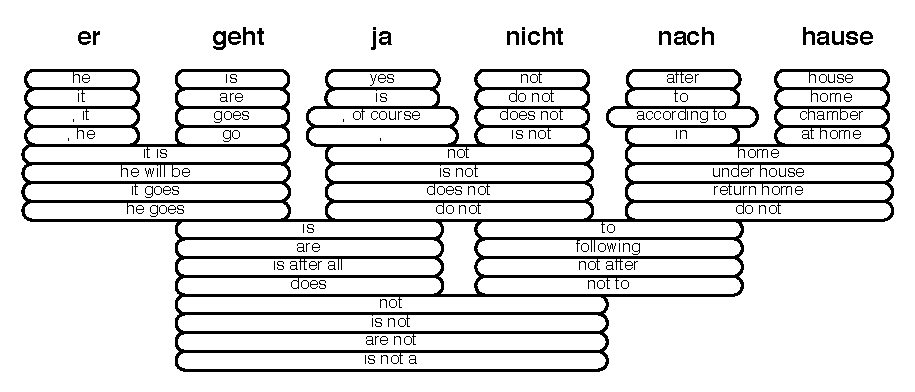
\includegraphics{g/translation-options.pdf}
 \caption{Translation Options}
 \caption*{\textit{\cite{Koehn2009a}}}
\end{figure}

This translation options are used as building blocks in process known as \textit{hypothesis expansion}. During this process, a data structure known as \textit{search graph} is being built by sequentially joining translation options that cover different parts of sentence in source language (Figure 2.2). Nodes of this graph are called \textit{hypotheses}. As new translation options are being added to existing hypotheses, new partial translation is formed \cite{Koehn2009a}. This process continues until sequence of hypotheses cover all parts of input sentence. Each hypothesis contains information about the translation being attached in current step, total score (based on log-probability) of current partial translation, link to previous hypothesis that is extended by current one and change in coverage vector of the foreign language sentence.


\begin{figure}
 \centering 
 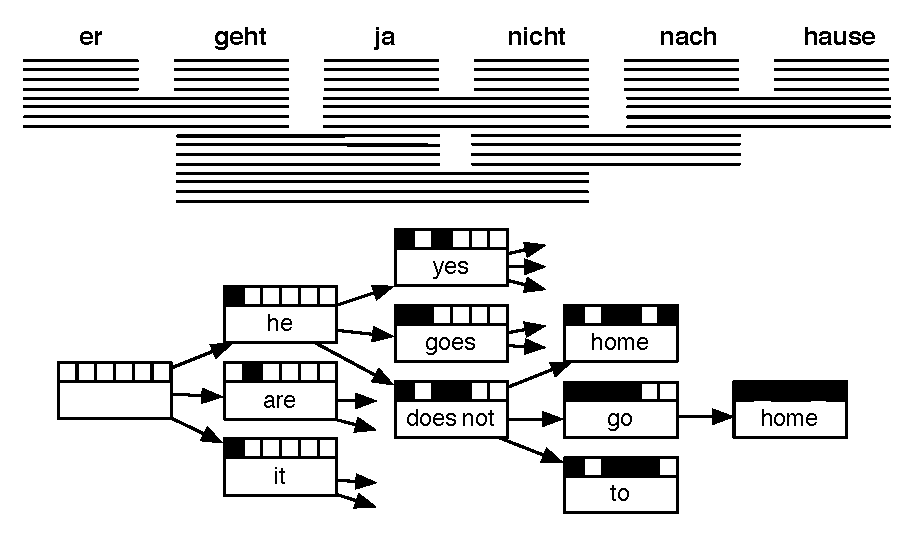
\includegraphics{g/decoding-step5.pdf}
 \caption{Hypothesis expansion}
 \caption*{\textit{\cite{Koehn2009a}}}
\end{figure}

\subsection{Hypothesis recombination}

The resulting data structure is still to large to be directly used for translation search. Several techniques are applied in order to reduce it's size. One way is using hypothesis recombination, which merges paths with same output and foreign language coverage. This reduction is risk-free and may not cause losing a good translation option. Sample of recombination is illustrated in Figures 2.3 and 2.4. Both hypotheses before recombination produce same output and cover same parts of source sentence, therefore the one with lower score could be recombined to reduce search space. Although this technique removes many unnecessary paths from graph, applying recombination doesn't affect overall exponential growth in number of hypothesis. 

\begin{figure}
 \centering 
 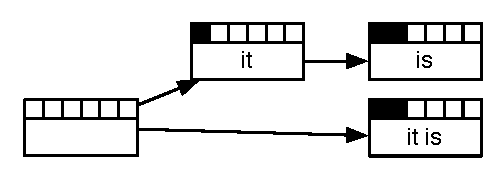
\includegraphics{g/recombination-example1.pdf}
 \caption{Before recombination}
 \caption*{\textit{\cite{Koehn2009a}}}
\end{figure}


\begin{figure}
 \centering 
 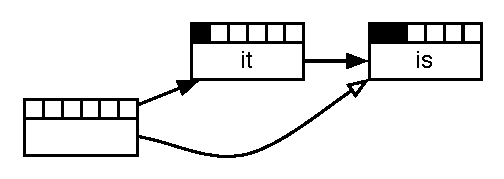
\includegraphics{g/recombination-example2.pdf}
 \caption{After recombination}
 \caption*{\textit{\cite{Koehn2009a}}}
\end{figure}


\subsection{Pruning}

Further reduction of search graph is required for longer sentences. \textit{Stack Decoding} is applied in order to filter hypothesis that have low probability of leading to good translations. Essential difference from recombination is that, this reduction technique is not risk-free and potentially may eliminate some useful translations. During this process stacks containing hypotheses with same coverage are constructed and pruning methods like histogram and threshold pruning are applied. As result number of items in stacks are reduced. 


\subsection{Summary}

In this section we provided a brief introduction into phrase-based Statistical Machine Translation, focusing on decoding stage during which search graph is being produced. Two main reasons of erroneous translation produced by the process described are \textit{search error} and \textit{model error}. While the first one corresponds to failure of finding correct translation during search, second one refers to initial problems in machine translation models. Assistance tool developed and investigated by us aims to provide users with an option to fix these errors within a CAT system by pointing to erroneous parts and selecting a better paraphrasing option from the list retrieved by the system. In some sense our approach lets user to reuse information collected during decoding. This information is available as search graph output, which optionally could be returned by Moses, together with translation results. 
